
\begin{figure}[h]
\centering


\tikzset{every picture/.style={line width=0.75pt}} %set default line width to 0.75pt        

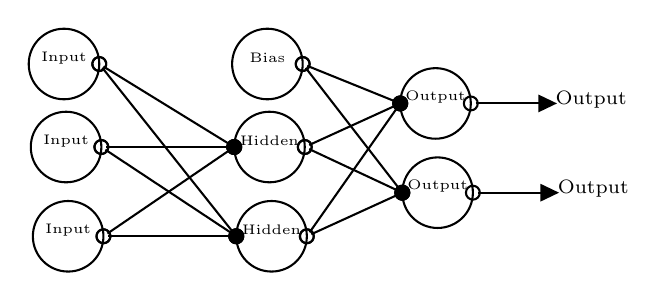
\begin{tikzpicture}[x=0.75pt,y=0.75pt,yscale=-1,xscale=1]
%uncomment if require: \path (0,300); %set diagram left start at 0, and has height of 300

\draw    (111, 77) circle [x radius= 17, y radius= 17]  ;
\draw    (130,78.23) -- (193,117) ;
\draw [shift={(193,117)}, rotate = 31.61] [color={rgb, 255:red, 0; green, 0; blue, 0 }  ][fill={rgb, 255:red, 0; green, 0; blue, 0 }  ][line width=0.75]      (0, 0) circle [x radius= 3.35, y radius= 3.35]   ;
\draw [shift={(128,77)}, rotate = 31.61] [color={rgb, 255:red, 0; green, 0; blue, 0 }  ][line width=0.75]      (0, 0) circle [x radius= 3.35, y radius= 3.35]   ;
\draw    (131.35,117) -- (193,117) ;
\draw [shift={(193,117)}, rotate = 0] [color={rgb, 255:red, 0; green, 0; blue, 0 }  ][fill={rgb, 255:red, 0; green, 0; blue, 0 }  ][line width=0.75]      (0, 0) circle [x radius= 3.35, y radius= 3.35]   ;
\draw [shift={(129,117)}, rotate = 0] [color={rgb, 255:red, 0; green, 0; blue, 0 }  ][line width=0.75]      (0, 0) circle [x radius= 3.35, y radius= 3.35]   ;
\draw    (131.94,158.68) -- (193,117) ;
\draw [shift={(193,117)}, rotate = 325.68] [color={rgb, 255:red, 0; green, 0; blue, 0 }  ][fill={rgb, 255:red, 0; green, 0; blue, 0 }  ][line width=0.75]      (0, 0) circle [x radius= 3.35, y radius= 3.35]   ;
\draw [shift={(130,160)}, rotate = 325.68] [color={rgb, 255:red, 0; green, 0; blue, 0 }  ][line width=0.75]      (0, 0) circle [x radius= 3.35, y radius= 3.35]   ;
\draw    (129.46,78.84) -- (194,160) ;
\draw [shift={(194,160)}, rotate = 51.51] [color={rgb, 255:red, 0; green, 0; blue, 0 }  ][fill={rgb, 255:red, 0; green, 0; blue, 0 }  ][line width=0.75]      (0, 0) circle [x radius= 3.35, y radius= 3.35]   ;
\draw [shift={(128,77)}, rotate = 51.51] [color={rgb, 255:red, 0; green, 0; blue, 0 }  ][line width=0.75]      (0, 0) circle [x radius= 3.35, y radius= 3.35]   ;
\draw    (130.96,118.3) -- (194,160) ;
\draw [shift={(194,160)}, rotate = 33.49] [color={rgb, 255:red, 0; green, 0; blue, 0 }  ][fill={rgb, 255:red, 0; green, 0; blue, 0 }  ][line width=0.75]      (0, 0) circle [x radius= 3.35, y radius= 3.35]   ;
\draw [shift={(129,117)}, rotate = 33.49] [color={rgb, 255:red, 0; green, 0; blue, 0 }  ][line width=0.75]      (0, 0) circle [x radius= 3.35, y radius= 3.35]   ;
\draw    (132.35,160) -- (194,160) ;
\draw [shift={(194,160)}, rotate = 0] [color={rgb, 255:red, 0; green, 0; blue, 0 }  ][fill={rgb, 255:red, 0; green, 0; blue, 0 }  ][line width=0.75]      (0, 0) circle [x radius= 3.35, y radius= 3.35]   ;
\draw [shift={(130,160)}, rotate = 0] [color={rgb, 255:red, 0; green, 0; blue, 0 }  ][line width=0.75]      (0, 0) circle [x radius= 3.35, y radius= 3.35]   ;
\draw    (112, 117) circle [x radius= 17, y radius= 17]  ;
\draw    (113, 160) circle [x radius= 17, y radius= 17]  ;
\draw    (209, 77) circle [x radius= 17, y radius= 17]  ;
\draw    (210, 117) circle [x radius= 17, y radius= 17]  ;
\draw    (211, 160) circle [x radius= 17, y radius= 17]  ;
\draw    (290, 96) circle [x radius= 17, y radius= 17]  ;
\draw    (291, 139) circle [x radius= 17, y radius= 17]  ;
\draw    (229.14,116.02) -- (273,96) ;
\draw [shift={(273,96)}, rotate = 335.46] [color={rgb, 255:red, 0; green, 0; blue, 0 }  ][fill={rgb, 255:red, 0; green, 0; blue, 0 }  ][line width=0.75]      (0, 0) circle [x radius= 3.35, y radius= 3.35]   ;
\draw [shift={(227,117)}, rotate = 335.46] [color={rgb, 255:red, 0; green, 0; blue, 0 }  ][line width=0.75]      (0, 0) circle [x radius= 3.35, y radius= 3.35]   ;
\draw    (229.13,118) -- (274,139) ;
\draw [shift={(274,139)}, rotate = 25.08] [color={rgb, 255:red, 0; green, 0; blue, 0 }  ][fill={rgb, 255:red, 0; green, 0; blue, 0 }  ][line width=0.75]      (0, 0) circle [x radius= 3.35, y radius= 3.35]   ;
\draw [shift={(227,117)}, rotate = 25.08] [color={rgb, 255:red, 0; green, 0; blue, 0 }  ][line width=0.75]      (0, 0) circle [x radius= 3.35, y radius= 3.35]   ;
\draw    (229.35,158.08) -- (273,96) ;
\draw [shift={(273,96)}, rotate = 305.11] [color={rgb, 255:red, 0; green, 0; blue, 0 }  ][fill={rgb, 255:red, 0; green, 0; blue, 0 }  ][line width=0.75]      (0, 0) circle [x radius= 3.35, y radius= 3.35]   ;
\draw [shift={(228,160)}, rotate = 305.11] [color={rgb, 255:red, 0; green, 0; blue, 0 }  ][line width=0.75]      (0, 0) circle [x radius= 3.35, y radius= 3.35]   ;
\draw    (230.14,159.02) -- (274,139) ;
\draw [shift={(274,139)}, rotate = 335.46] [color={rgb, 255:red, 0; green, 0; blue, 0 }  ][fill={rgb, 255:red, 0; green, 0; blue, 0 }  ][line width=0.75]      (0, 0) circle [x radius= 3.35, y radius= 3.35]   ;
\draw [shift={(228,160)}, rotate = 335.46] [color={rgb, 255:red, 0; green, 0; blue, 0 }  ][line width=0.75]      (0, 0) circle [x radius= 3.35, y radius= 3.35]   ;
\draw    (228.18,77.88) -- (273,96) ;
\draw [shift={(273,96)}, rotate = 22.01] [color={rgb, 255:red, 0; green, 0; blue, 0 }  ][fill={rgb, 255:red, 0; green, 0; blue, 0 }  ][line width=0.75]      (0, 0) circle [x radius= 3.35, y radius= 3.35]   ;
\draw [shift={(226,77)}, rotate = 22.01] [color={rgb, 255:red, 0; green, 0; blue, 0 }  ][line width=0.75]      (0, 0) circle [x radius= 3.35, y radius= 3.35]   ;
\draw    (227.44,78.86) -- (274,139) ;
\draw [shift={(274,139)}, rotate = 52.25] [color={rgb, 255:red, 0; green, 0; blue, 0 }  ][fill={rgb, 255:red, 0; green, 0; blue, 0 }  ][line width=0.75]      (0, 0) circle [x radius= 3.35, y radius= 3.35]   ;
\draw [shift={(226,77)}, rotate = 52.25] [color={rgb, 255:red, 0; green, 0; blue, 0 }  ][line width=0.75]      (0, 0) circle [x radius= 3.35, y radius= 3.35]   ;
\draw    (309.35,96) -- (346.5,96) ;
\draw [shift={(348.5,96)}, rotate = 180] [fill={rgb, 255:red, 0; green, 0; blue, 0 }  ][line width=0.75]  [draw opacity=0] (8.93,-4.29) -- (0,0) -- (8.93,4.29) -- cycle    ;
\draw [shift={(307,96)}, rotate = 0] [color={rgb, 255:red, 0; green, 0; blue, 0 }  ][line width=0.75]      (0, 0) circle [x radius= 3.35, y radius= 3.35]   ;
\draw    (310.35,139) -- (347.5,139) ;
\draw [shift={(349.5,139)}, rotate = 180] [fill={rgb, 255:red, 0; green, 0; blue, 0 }  ][line width=0.75]  [draw opacity=0] (8.93,-4.29) -- (0,0) -- (8.93,4.29) -- cycle    ;
\draw [shift={(308,139)}, rotate = 0] [color={rgb, 255:red, 0; green, 0; blue, 0 }  ][line width=0.75]      (0, 0) circle [x radius= 3.35, y radius= 3.35]   ;

\draw (111,74) node  [align=left] {{\tiny Input}};
\draw (112,114) node  [align=left] {{\tiny Input}};
\draw (113,157) node  [align=left] {{\tiny Input}};
\draw (209,74) node  [align=left] {{\tiny Bias}};
\draw (210,114) node  [align=left] {{\tiny Hidden}};
\draw (211,157) node  [align=left] {{\tiny Hidden}};
\draw (290,93) node  [align=left] {{\tiny Output}};
\draw (291,136) node  [align=left] {{\tiny Output}};
\draw (365,94) node  [align=left] {{\scriptsize Output}};
\draw (366,137) node  [align=left] {{\scriptsize Output}};


\end{tikzpicture}
\caption{An example of a feedforward neural network}
\subcaption{Note than an empty circle on an edge denotes a source and a filled circle on an edge denotes a sink.}
\end{figure}